\documentclass{beamer} 
\usetheme{Boadilla} 
\usepackage{amsmath,amsfonts,amsthm,amssymb, amscd}
\usepackage{setspace}
\usepackage{Tabbing}
\usepackage{fancyhdr}
\usepackage{lastpage}
\title{The Beginning of Awesomeness}
\author{Lalit}
\institute{UW-Madison}


\begin{document}
\begin{frame}
  \titlepage
  
\end{frame}

\begin{frame}
\frametitle{Outline}
\tableofcontents[pausesections]
\end{frame}


%%%%%%%%%%%%%%%%%%%%%%%%%%%%%%%%%%%%%%%%%%%%%%%%%%%%%%%%%%%%%%%%%%%%%%%%%
\section{Introduction}
\begin{frame}
\frametitle{Introduction}
\LaTeX is a document creation tool that will rock your world!!!
\pause
\begin{center}
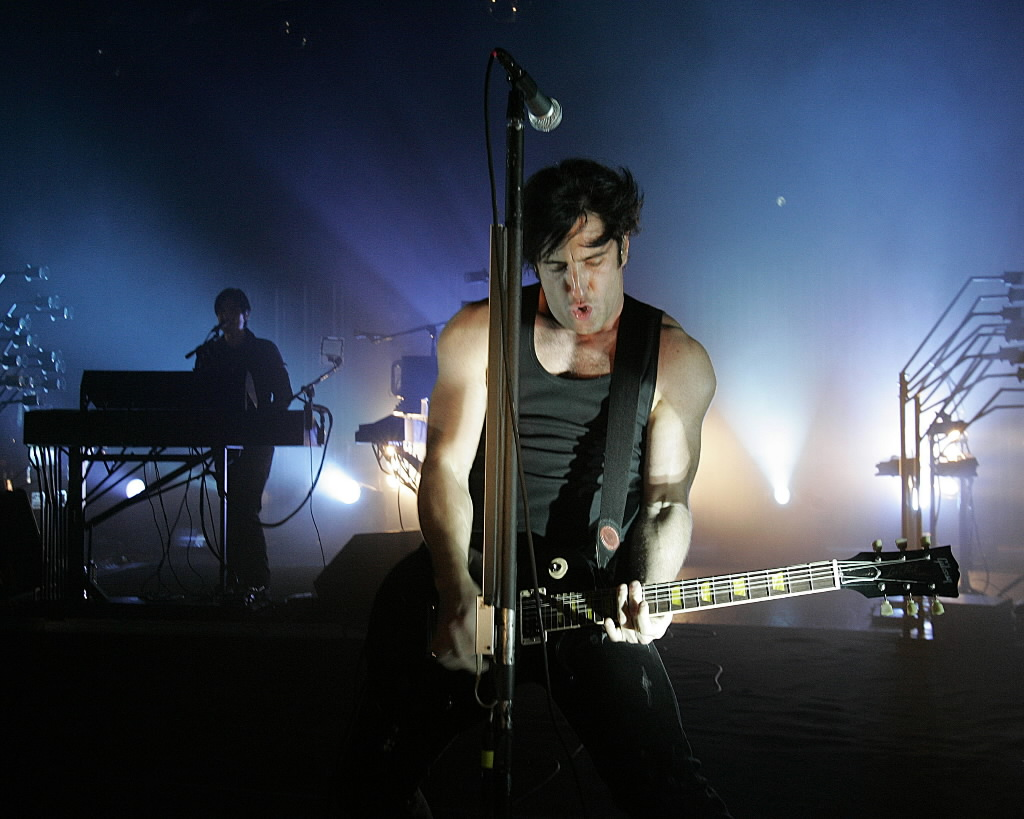
\includegraphics[scale=.25]{rock.jpg}
\end{center}
\end{frame}

\begin{frame}
\frametitle{Terminology}
Note: Pronounced "Latec" not "Latex." 

\begin{center}
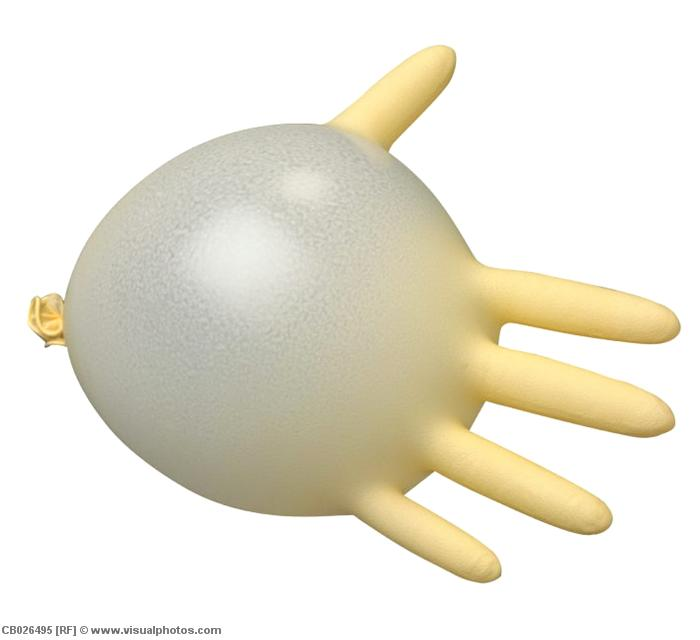
\includegraphics[scale=.4]{gloves.jpg}
\end{center}
\end{frame}

%%%%%%%%%%%%%%%%%%%%%%%%%%%%%%%%%%%%%%%%%%%%%%%%%%%%%%%%%%%%%%%%%%%%%%%
\section{How Things Fit Together}
\begin{frame}
\frametitle{Components}
There are three different things to keep separate in your head:
\setbeamercovered{transparent}
\begin{itemize}
\item<1> \LaTeX
\item<2> Beamer
\item<3> The editor you use.
\end{itemize}
You could always prepare \LaTeX in a text file and run latex on it.
\end{frame}

\begin{frame}
\frametitle{I Don't Like Microsoft Products}
\LaTeX is the most widely used tool for math and science typsetting.
\pause
\vspace{20mm}
Word and Powerpoint suck. 
\pause
\end{frame}

%%%%%%%%%%%%%%%%%%%%%%%%%%%%%%%%%%%%%%%%%%%%%%%%%%%%%%%%%%%%%%%%%%%%%%
\section{Examples and References}
\begin{frame}
You can put math {\it inline}, like this: $x^2=4\rightarrow x=\pm 2.$

Or like this:
$$ \int_0^1 x^2 dx = \frac{1}{3}$$
Or you can show somebody the steps of a computation:
\begin{align*}
\int_0^1 x^2 dx &= \left.\frac{x^3}{3}\right|_0^1\\
&= \frac{1}{3}
\end{align*}
\end{frame}

\begin{frame}
\LaTeX resources:
\begin{itemize}
\item\href{http://www.artofproblemsolving.com/Wiki/index.php/LaTeX:About}{AOPS Guide}
\item\href{http://www.artofproblemsolving.com/Wiki/index.php/LaTeX:Symbols}{Latex Symbols}
\end{itemize}
Beamer Resources:
\begin{itemize}
\item \href{http://www.tug.org/pracjourn/2005-4/mertz/mertz.pdf}{Lots of Examples}
\item \href{http://www.uncg.edu/cmp/reu/presentations/CharlesBatts-BeamerTutorial.pdf}{Also Down to Earth}
\item \href{http://en.wikibooks.org/wiki/LaTeX/Presentations}{I liked this one too.}
\item \href{http://www.math.umbc.edu/~rouben/beamer/}{Technical Overview}
\item \href{http://www.tug.org/teTeX/tetex-texmfdist/doc/latex/beamer/beameruserguide.pdf}{The Official User Guide}
\end{itemize}
\end{frame}
%%%%%%%%%%%%%%%%%%%%%%%%%%%%%%%%%%%%%%%%%%%%%%%%%%%%%%%%%%%%%%%%%%%%%%%%%
\section{Your Turn!}
\begin{frame}
Your Task for the day:
\begin{itemize}
\item Create a short presentation on Groups.
\item State the definition, and one theorem.
\item Have 5-10 slides.
\item Use inline and non-inline math.
\item Use an {\texttt align} somewhere.
\item Use overlays.
\item Make Beamer look good. Use a different theme:\href{See This}{http://www.math.umbc.edu/~rouben/beamer/}
\item Bonus: Include a sweet picture.
\end{itemize}
\end{frame}

\end{document}
